% Created 2018-06-08 Fri 18:15
\documentclass[9pt, b5paper]{article}
\usepackage{fontspec}
\usepackage{graphicx}
\usepackage{xcolor}
\usepackage[slantfont,boldfont]{xeCJK}
\setCJKmainfont[BoldFont = Heiti SC, ItalicFont = STFangsong]{STSong}
\setCJKsansfont{STHeiti}
\setCJKmonofont{STFangsong}
\usepackage{multirow}
\usepackage{multicol}
\usepackage{float}
\usepackage{textcomp}
\usepackage{geometry}
\geometry{left=0.1cm,right=0.1cm,top=0.1cm,bottom=0.1cm}
\usepackage{algorithm}
\usepackage{algorithmic}
\usepackage{latexsym}
\usepackage{natbib}
\usepackage{listings}
\usepackage{minted}
\usepackage[xetex,colorlinks=true,CJKbookmarks=true,linkcolor=blue,urlcolor=blue,menucolor=blue]{hyperref}
\author{黄和燕}
\date{\today}
\title{Unity ShaderLab学习总结 -- deeper}
\hypersetup{
  pdfkeywords={},
  pdfsubject={},
  pdfcreator={Emacs 25.3.1 (Org mode 8.2.7c)}}
\begin{document}

\maketitle
\tableofcontents


\section{Unity3D Shader基础学习(一):Shader基础知识}
\label{sec-1}
\begin{itemize}
\item \url{http://gad.qq.com/article/detail/28617}
\item 这是一个Unity3d Shader 学习系列,是会对Unity Shader相关的进行简单的探讨学习,对于资深开发人士来说,这个系列可能比较表层,但对于不是专门做Shader方面的来说,能够简单学习到里面所实现的原理,并理解它也是很厉害的了。
\item 对于Shader,可能有些人会有些陌生,翻译一下就是着色器的意思,我们可以通过不同硬件所支持的不同的着色器语言可以来实现我们需要的图形效果。如果读者学过计算机图形学,相信对着色器并不会陌生。关于Shader的简介,这里就不多介绍。
\item Unity中,可以使用哪种Shader语言来编写呢,其实使用哪种语言都可以编写Shader,比如英伟达公司的CG,微软的HLSL以及SGI公司的GLSL语言都是可以的,具体使用什么语言来开发,就根据开发者开发中所支持的目标平台的不同来决定。而Unity中又对这些不同硬件所支持的不同Shader进行了统一的封装,我们只要按照它所封装好的规则来编写,就可以实现不同平台的支持,我们这里把这个封装所写的Shader称为ShaderLab。话不多说,我们现在就开始编写Unity中最简单的一个ShaderLab。
\begin{minted}[linenos=true]{csharp}
// Shader模块定义  
Shader "xiaolezi/SimpleShader" {
    // 属性设置  
    Properties {
        // 定义物体表面颜色,格式:[属性名]([Inspector面板显示名字],属性类型)=[初始值]  
        _Color("Tint Color", Color) = (1,1,1,1)  
    }  
    // 第一个SubShader块  
    SubShader {  
        // 第一个Pass块  
        Pass {  
            // 开启CG着色器编辑模块  
            CGPROGRAM  
            // 定义顶点着手器函数名  
            #pragma vertex vert  
            // 定义片段着色器函数名  
            #pragma fragment frag  
            // 定义一个从应用程序到顶点数据的结构体  
            struct appdata {  
                float4 vertex : POSITION;// POSITION语义:表示从该模型中获取到顶点数据  
            };  
            // 定义一个从顶点数据到片段数据的结构体  
            struct v2f {  
                // SV_POSITION语义:得到输入片元着色器中的顶点数据  
                float4 vertex : SV_POSITION;
            };  
            // 从属性模块中取得该变量  
            fixed4 _Color;  
            // 顶点着色器函数实现  
            v2f vert(appdata v) {  
                v2f o;  
                // 让模型顶点数据坐标从本地坐标转化为屏幕剪裁坐标  
                o.vertex = UnityObjectToClipPos(v.vertex);
                return o;  
            }  
            // 片段着色器函数实现  
            // SV_Target语义:输出片元着色器值,可直接认为是输出到屏幕颜色
            fixed4 frag(v2f i) : SV_Target {  
                return _Color;  
        }  
        // 结束CG着色器编辑模块  
        ENDCG  
        }  
    }  
}
\end{minted}
\item 看起来挺复杂的,不过不要担心,我们一个个来分析。
\item 首先我们先来了解一下关于ShaderLab的一个模板,如下:
\begin{minted}[linenos=true]{csharp}
Shader "名称/.."{  
    Properties{  
        // ...  
    }  
    SubShader{  
        Pass{  
            CGPROGRAM  
            // ...  
            ENDCG  
        }  
    }  
    Fallback "默认着色器"  
}
\end{minted}
\item 这个模板就是ShaderLab封装的一个模板,我们以后就会根据这个模板来编写我们的shader。
\item 我们再来了解一下几个关键字:
\begin{itemize}
\item Shader关键字,后面跟着一条字符串,当你在材质选择面板时,你可以通过使用正斜杠符"/"在子集菜单放置你的shader文件。
\item Properties关键字,在语句块中包含了shader的变量,例如(color,texture等等),它将会保存在我们的材质中,并且显示在材质面板上。
\item SubShader关键字,着色器中可以包含一个或多个Shader文件,它会根据不同的GPU的兼容来决定使用那个SubShader。
\item Pass关键字,每个SubShader会编写很多Pass块,每个Pass块代表对拥有相同着色器材质被渲染的对象的一个可执行的顶点片元代码。很多简单的着色器只使用一个Pass,但是对于一些被光照相互的着色器就需要多个Pass。Pass中的一个名字通常会设置一些固定功能的状态,比如混合模式,这个后面再探讨。
\item CGPROGRAM\ldots{}ENDCG关键字:顶点片元着色器代码需要写在这两个关键字里面。
\end{itemize}
\item 好,我们现在来分析一下上面所给的代码。
\begin{minted}[linenos=true]{csharp}
Shader "xiaolezi/SimpleShader"
\end{minted}
\item 这里我定义了我的材质面板所存放该shader的目录,如图:
\begin{minted}[linenos=true]{csharp}
// 属性设置  
Properties {  
    // 定义一个物体表面颜色,格式:[属性名]([Inspector面板显示名字],属性类型)=[初始值]  
    _Color("Tint Color", Color) = (1, 1, 1, 1)  
}
\end{minted}
\item 这里定义了一个颜色属性,关于属性类型,还有哪一些呢,我们常有的有以下种:
\begin{itemize}
\item 整型 Int
\item 浮点型 Float
\item 随机数 Range(min,max)
\item 颜色属性 Color
\item 向量属性 Vector
\item 纹理属性 2D 3D Cube
\end{itemize}
\item 具体我们到时用到再说。
\item 然后我们再来看看Pass语句下的顶点片元函数的实现:
\item 首先我们需要定义顶点片元着色器函数,通过如下代码定义:
\begin{minted}[linenos=true]{csharp}
 #pragma vertex vert  
 #pragma fragment frag
\end{minted}
\item vert和frag分别为它们的函数名,这个可以自定义。
\item 然后我们需要对顶点片元函数进行实现,而实现之前需要定义相关结构体来得到一些相关值。
\item 所以,这里还要对渲染管线进行分析,我们来看一张图简单了解一下关于GPU是怎么对图像进行渲染的:

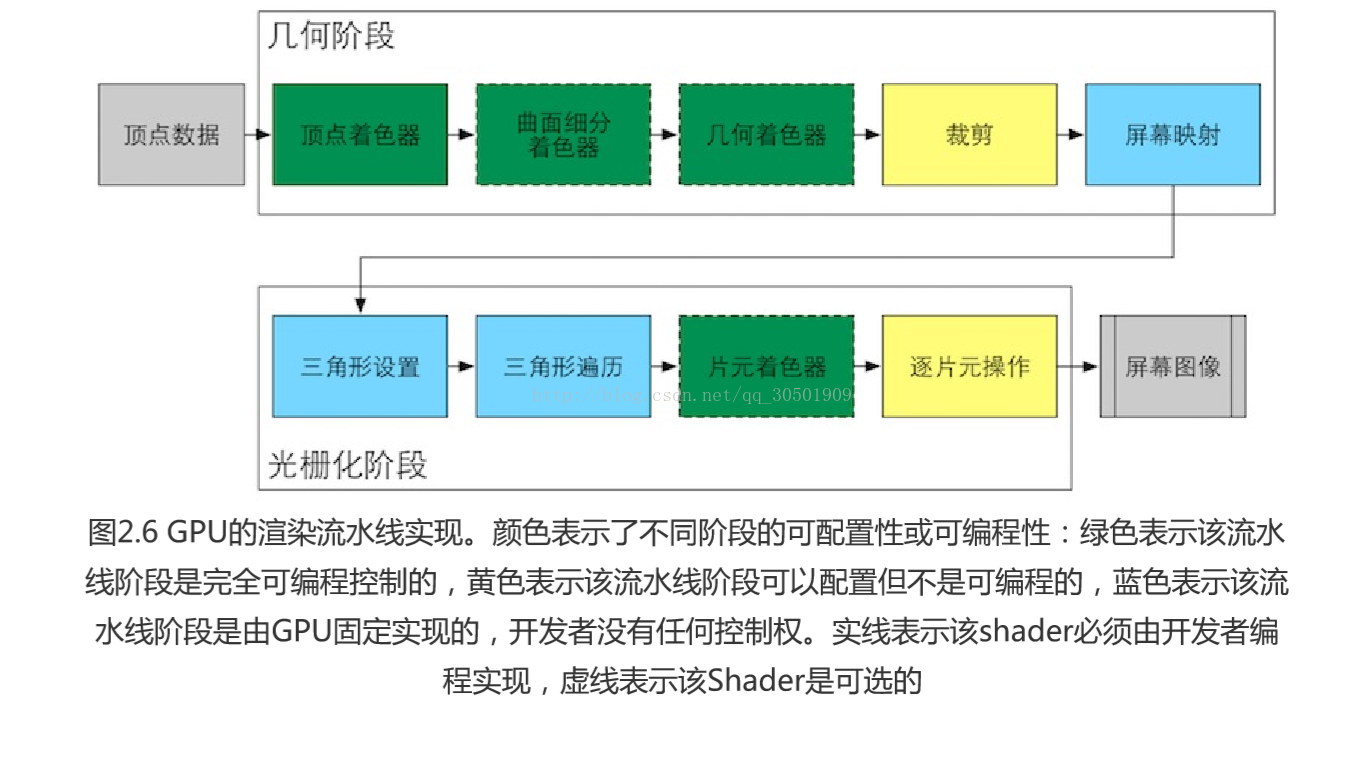
\includegraphics[width=.9\linewidth]{./pic/process.png}
\item 我们知道,想要图像完整的被硬件所渲染,其实步骤还是很复杂的。首先要获取顶点数据,再通过几何光栅化阶段最终才能获得我们的屏幕图像。之前硬件限制,实现的Shader是固定的渲染管线,基本很多不可编程的,所以实现起来也很麻烦。现在的Shader很多可以编程,这样让Shader实现起来会很方便。所以我们现在所实现的过程就是上面绿色部分当中的内容。
\item 好,我们这里关注点有两个,一个是顶点着色器,一个是片元着色器。这里有两个问题:
\begin{itemize}
\item 1.顶点数据在Unity中从哪里获取得到;
\item 2.顶点数据在怎么输入与输出到顶点着色器和片段着色器中。
\end{itemize}
\item 我们先来解决第一个问题,Unity中,获取顶点数据会从当前物体的Mesh Filter组件中获取得到,这里面保存了大量的顶点信息。我们在Wireframe模式下观察各个顶点的连线信息,如图所示:
\item Unity3D Shader基础学习(一):Shader基础知识
\item 第二个问题,顶点信息是怎么输入和输出的,这里通过语义(Semantics)来获取和输出。
\item 在顶点着色器中,我们可以使用哪些语义来得到顶点数据呢?如下:
\begin{itemize}
\item POSITION 顶点位置,一般为一个float3或float4类型
\item NORMAL 顶点法线,一般为一个float3类型
\item TEXCOORD0 纹理坐标,一般为float2,float3或float4类型
\item TEXCOORD1, TEXCOORD2 and TEXCOORD3 分别是 第二,第三,第四级纹理坐标
\item TANGENT 切线向量(通常被使用作为法线贴图),一般为float4类型
\item COLOR 逐顶点颜色,一般为float4类型
\end{itemize}
\item 而片元着色器中,可以使用以下语义获得顶点数据:
\begin{itemize}
\item SV$_{\text{POSITION}}$
\item COLOR0 Color1
\item TEXCOORD0\textasciitilde{}7
\end{itemize}
\item 最终从片元着色器中输出的语义为:
\begin{itemize}
\item SV$_{\text{Target}}$
\end{itemize}
\item 好,现在继续再来看看我们的代码,先来看看这两个结构体:
\begin{minted}[linenos=true]{csharp}
// 定义一个从应用程序到顶点数据的结构体  
struct appdata {
    // POSITION语义:表示从该模型中获取到顶点数据      
    float4 vertex : POSITION;
};  
// 定义一个从顶点数据到片段数据的结构体  
struct v2f {
    // SV_POSITION语义:得到输入片元着色器中的顶点数据  
    float4 vertex : SV_POSITION;
};
\end{minted}
\item 一个是需要在顶点着色器中使用的,所以我们定义的结构体需要使用顶点着色器中的获取顶点数据的语义,这里通过POSITION得到了顶点位置信息,是模型空间下的。
\item 接着,第二个结构体是需要在片元着色器中使用的,所以我们也是需要使用片元着色器获取顶点数据的语义,这里也是得到顶点数据。
\item 好,最后来看下顶点片元函数的实现了:
\begin{minted}[linenos=true]{csharp}
// 从属性模块中取得该变量  
fixed4 _Color;  
// 顶点着色器函数实现  
v2f vert(appdata v) {  
    v2f o;
    // 让模型顶点数据坐标从本地坐标转化为屏幕剪裁坐标      
    o.vertex = UnityObjectToClipPos(v.vertex);
    return o;  
}  
// 片段着色器函数实现
// SV_Target语义:输出片元着色器值,可直接认为是输出到屏幕颜色 
fixed4 frag(v2f i) : SV_Target {
    return _Color;  
}
\end{minted}
\item 首先,我们看下第一行,取得变量$_{\text{Color}}$,虽然我们的变量在属性面板中有定义,但是如果要在Pass中使用,你就必须重新定义一下,这是Shader和其他高级语言不一样的地方。所以这一点知道就好。
\item 然后 顶点着色器函数返回我们的片元着色器结构体数据,自然,在函数中需要定义一个片元着色器结构体,然后关键的一步就是把你通过POSITION语义去的顶点位置信息从模型空间转化为剪裁空间。上面的渲染管线图有这具体的一步。而在Unity中,只要调用封装好的这个方法UnityObjectToClipPos,然后把顶点坐标传入即可,接着我们把它转化后的坐标保存在o这个结构体中方便在片元着色器中访问得到。
\item 片元着色器中,需要返回具体的图像颜色值,所以我们设置返回值为 fixed4这个类型,然后直接把我们当前属性的颜色返回。一般,颜色值得数据都设置为fixed类型,这样对性能好一些。
\item 以上就是对Shader中最基本编写进行解剖。希望能够启发读者对Unity中Shader的使用。
\end{itemize}

\section{Unity3d Shader基础学习(二):漫反射}
\label{sec-2}
\begin{itemize}
\item - \url{http://gad.qq.com/article/detail/28618}
\item 上一篇我们了解了Unity中Shader相关介绍以及实现了一个最简单的Shader。
\item 这一篇我们会学习中更为立体的Shader,即通过光照计算物体表面的漫反色。这里,我们通过兰伯特光照模型原理实现物体漫反色原理。关于标准光照模型,我们留在下次再介绍。好,先来看看我们这次所实现效果:
\item 可能录制时采样问题,我这里再提供一张静态图。
\item 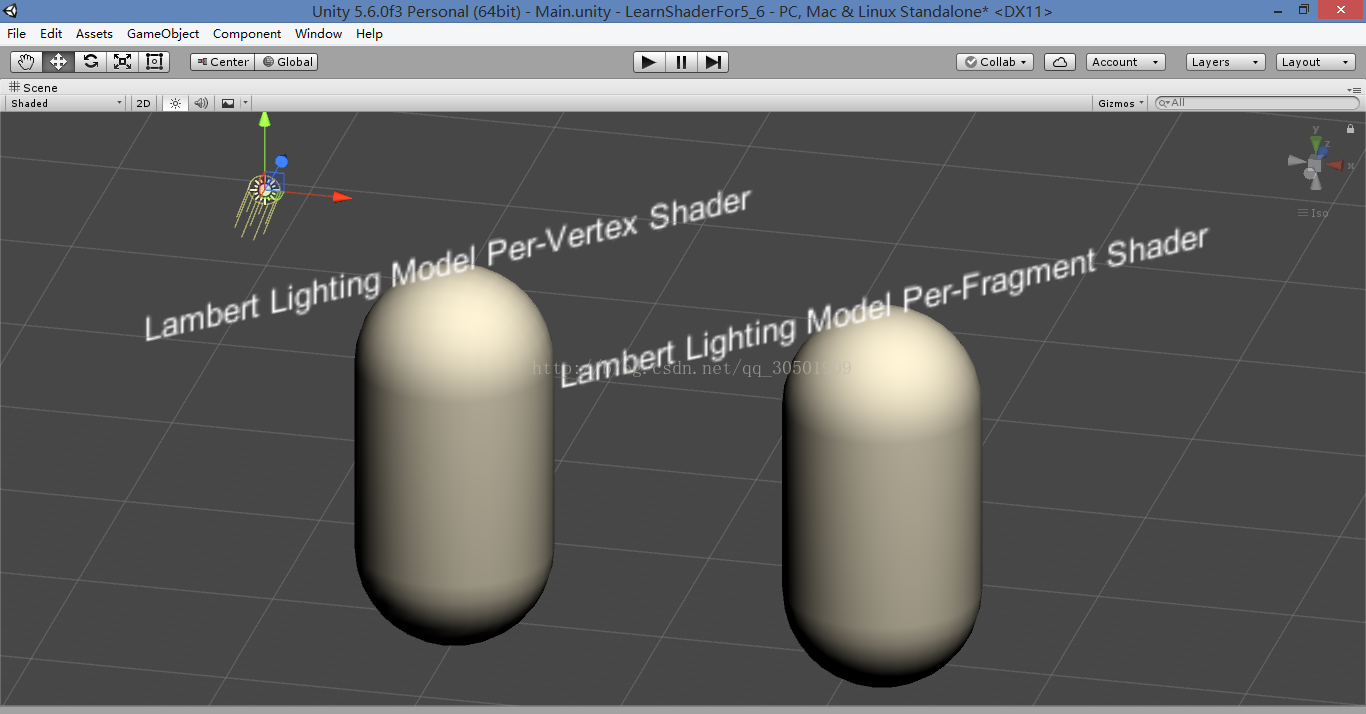
\includegraphics[width=.9\linewidth]{./pic/shader-compare.png}
\item 这里我实现了关于逐顶点和逐像素的漫反射,虽然看起来感觉差不多,但是还是有细微的区别,毕竟处理方式不同,相对逐顶点而言,逐像素看起来会更柔化一些。
\item 好,我们再来看看代码实现,先看逐顶点:
\begin{minted}[linenos=true]{csharp}
// Shader模块定义  
Shader "xiaolezi/Lambert Lighting Model Per-Vertex Shader" {  
    // 属性设置  
    Properties {  
        // 定义一个物体表面颜色,格式:[属性名]([Inspector面板显示名字],属性类型)=[初始值]  
        _DiffuseColor("Diffuse Color", Color) = (1, 1, 1, 1)  
    }  
    // 第一个SubShader块  
    SubShader {  
        // 第一个Pass块  
        Pass {  
            // 指定灯光渲染模式  
            Tags{ "LightMode" = "ForwardBase" }  
            // 开启CG着色器编辑模块  
            CGPROGRAM  
            // 定义顶点着手器函数名  
            #pragma vertex vert  
            // 定义片段着色器函数名  
            #pragma fragment frag  
            // 包含相关头文件  
            #include "UnityCG.cginc"      
            #include "Lighting.cginc"  
            // 定义一个从应用程序到顶点数据的结构体  
            struct appdata {  
                float4 vertex : POSITION; // POSITION语义:表示从该模型中获取到顶点数据  
                float3 normal : NORMAL;   // NORMAL语义:获取该模型法线  
            };  
            // 定义一个从顶点数据到片段数据的结构体  
            struct v2f {  
                float4 pos : SV_POSITION; // SV_POSITION语义:从顶点输出数据中获取到顶点数据  
                fixed3 diffuse : COLOR0;  // COLOR0语义:定义颜色信息  
            };  
            // 从属性模块中取得该变量  
            fixed4 _DiffuseColor;  
            // 顶点着色器函数实现  
            v2f vert(appdata v) {  
                v2f o;  
                o.pos = UnityObjectToClipPos(v.vertex);// 让模型顶点数据坐标从本地坐标转化为屏幕剪裁坐标  
                fixed3 normalDir = normalize(UnityObjectToWorldNormal(v.normal));// 计算世界法线方向  
                fixed3 lightDir = normalize(ObjSpaceLightDir(v.vertex));   // 计算灯光方向  
                float Lambert = max(dot(normalDir, lightDir), 0);          // 兰伯特值  
                o.diffuse = _LightColor0.rgb * _DiffuseColor.rgb * Lambert;// 计算漫反色  
                return o;  
            }  
            // 片段着色器函数实现
            fixed4 frag(v2f f) : SV_Target { 
                // SV_Target语义:输出片元着色器值,可直接认为是输出到屏幕颜色             
                return fixed4(f.diffuse, 1.0);  
            }  
            // 结束CG着色器编辑模块  
            ENDCG  
        }  
    }  
    Fallback "Diffuse"// 默认着色器  
}
\end{minted}
\item 接着是逐像素:
\begin{minted}[linenos=true]{csharp}
// Shader模块定义  
Shader "xiaolezi/Lambert Lighting Model Per-Fragment Shader" {  
    // 属性设置  
    Properties {  
        // 定义一个物体表面颜色,格式:[属性名]([Inspector面板显示名字],属性类型)=[初始值]  
        _DiffuseColor("Diffuse Color", Color) = (1, 1, 1, 1)  
    }  
    // 第一个SubShader块  
    SubShader {  
        // 第一个Pass块  
        Pass {  
            // 指定灯光渲染模式  
            Tags{ "LightMode" = "ForwardBase" }  
            // 开启CG着色器编辑模块  
            CGPROGRAM  
            // 定义顶点着手器函数名  
            #pragma vertex vert  
            // 定义片段着色器函数名  
            #pragma fragment frag  
            // 包含相关头文件  
            #include "UnityCG.cginc"      
            #include "Lighting.cginc"  
            // 定义一个从应用程序到顶点数据的结构体  
            struct appdata {  
                float4 vertex : POSITION; // POSITION语义:表示从该模型中获取到顶点数据  
                float3 normal : NORMAL;   // NORMAL语义:获取该模型法线  
            };  
            // 定义一个从顶点数据到片段数据的结构体  
            struct v2f {  
                float4 pos : SV_POSITION; // SV_POSITION语义:从顶点输出数据中获取到顶点数据  
                float3 normal : COLOR0;   // COLOR0语义:定义法线变量  
                float4 vertex : COLOR1;   // COLOR1语义:定义顶点变量  
            };  
            // 从属性模块中取得该变量  
            fixed4 _DiffuseColor;  
            // 顶点着色器函数实现  
            v2f vert(appdata v) {  
                v2f o;
                // 让模型顶点数据坐标从本地坐标转化为屏幕剪裁坐标  
                o.pos = UnityObjectToClipPos(v.vertex); 
                o.normal = v.normal;  
                o.vertex = v.vertex;  
                return o;  
            }  
            // 片段着色器函数实现  
            fixed4 frag(v2f f) : SV_Target {
                // SV_Target语义:输出片元着色器值,可直接认为是输出到屏幕颜色
                fixed3 normalDir = normalize(UnityObjectToWorldNormal(f.normal)); // 计算世界法线方向  
                fixed3 lightDir = normalize(ObjSpaceLightDir(f.vertex));          // 计算灯光方向  
                float Lambert = max(dot(normalDir, lightDir), 0);                 // 兰伯特值  
                fixed3 diffuse = _LightColor0.rgb * _DiffuseColor.rgb * Lambert;  // 计算漫反色  
                return fixed4(diffuse, 1.0);  
            }  
            // 结束CG着色器编辑模块  
            ENDCG  
        }  
    }  
    Fallback "Diffuse"// 默认着色器  
}
\end{minted}
\item 好,现在我们先不解释上述代码,我们先来了解一下兰伯特光照原理。先来看一张图:

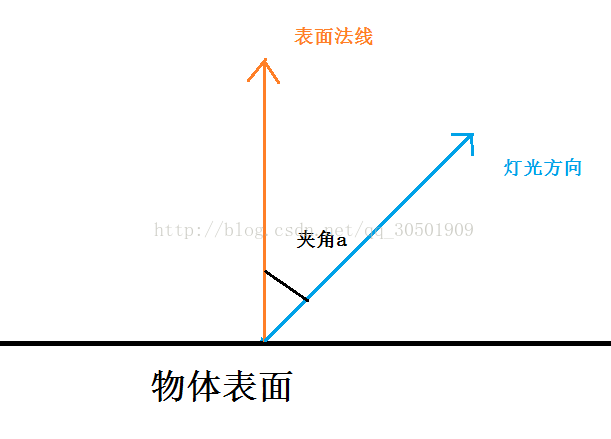
\includegraphics[width=.9\linewidth]{./pic/lambert.png}
\item 其实我们兰伯特计算原理就是法线方向向量与灯光方向向量的点积,即兰伯特值Lambert = NormalDir * LightDir *Cos(夹角a)。由此我们可以得知,夹角越大,兰伯特值越大,物体表面越亮。
\item 知道兰伯特原理之后,我们就可以来直接看代码了,基本的那些代码就不多说,注释也有说明,我们来看看不一样的地方。
\item 先来看逐顶点着色器部分,逐顶点的是指把所有颜色相关计算都在顶点着色器中计算,而最终通过一个颜色变量传递给片元着色器直接输出。我们直接来看Pass语句块实现原理。
\item 第一行代码:
\begin{minted}[linenos=true]{csharp}
//指定灯光渲染模式  
Tags{"LightMode" = "ForwardBase"}
\end{minted}
\item 首先,因为考虑到灯光颜色对物体影响,我们需要得到灯光的变量$_{\text{LightColor0。而这个变量虽然可以通过包含灯光文件}}$"Lighting.cginc"来获取得到,但是如果没有指定灯光的渲染模式,该变量并不能正确被赋值,那么在计算的时候,就会导致实现的效果与预期效果有所偏差,这也不是我们所想要的结果。
\item 接着,引入两个头文件,可以通过所引入头文件获取当中相关变量和方法。
\begin{minted}[linenos=true]{csharp}
//包含相关头文件  
#include "UnityCG.cginc"      
#include "Lighting.cginc"
\end{minted}
\item 这里建议读者有空可以多去看看Unity中相关的CG头文件里的内容,具体目录在:
\begin{minted}[linenos=true]{csharp}
"安装目录/Unity/Editor/Data/CGIncludes/"
\end{minted}
\item 如上面的"UnityCG.cginc",里面有相关坐标的转化,例如:我们上述代码中所实现的ObjSpaceLightDir方法,UnityObjectToWorldNormal方法,都是在当中定义实现的,是相当值得一看的,这里就不多介绍了。
\item 然后,我们来看看我们的顶点函数中所实现的兰伯特值:
\begin{minted}[linenos=true]{csharp}
// 顶点着色器函数实现  
v2f vert(appdata v) {  
    v2f o;  // 让模型顶点数据坐标从本地坐标转化为屏幕剪裁坐标  
    o.pos = UnityObjectToClipPos(v.vertex); 
    fixed3 normalDir = normalize(UnityObjectToWorldNormal(v.normal)); // 计算世界法线方向  
    fixed3 lightDir = normalize(ObjSpaceLightDir(v.vertex));          // 计算灯光方向  
    float Lambert = max(dot(normalDir, lightDir), 0);                 // 兰伯特值  
    o.diffuse = _LightColor0.rgb * _DiffuseColor.rgb * Lambert;       // 计算漫反色  
    return o;  
}
\end{minted}
\item 因为计算兰伯特值需要得到法线和光照两个方向向量,而法线可以通过模型法线转换得到,光照向量可以由模型顶点得到,所以我们需要在顶点结构体中定义了一个法线语义来获取模型法线:
\begin{minted}[linenos=true]{csharp}
// 定义一个从应用程序到顶点数据的结构体  
struct appdata {  
    float4 vertex : POSITION; // POSITION语义:表示从该模型中获取到顶点数据  
    float3 normal : NORMAL;   // NORMAL语义:获取该模型法线  
};
\end{minted}
\item 在计算完兰伯特值之后,就可以计算物体的漫反色颜色值了,计算完成之后,我们需要在片元结构体中定义一个漫反色值来存储该颜色值:
\begin{minted}[linenos=true]{csharp}
// 定义一个从顶点数据到片段数据的结构体  
struct v2f {  
    float4 pos : SV_POSITION; // SV_POSITION语义:从顶点输出数据中获取到顶点数据  
    fixed3 diffuse : COLOR0;  // COLOR0语义:定义颜色信息  
};
\end{minted}
\item 最后,我们在片元函数中直接输出该漫反色值即可:
\begin{minted}[linenos=true]{csharp}
// 片段着色器函数实现  
fixed4 frag(v2f f) : SV_Target {
    // SV_Target语义:输出片元着色器值,可直接认为是输出到屏幕颜色  
    return fixed4(f.diffuse, 1.0);  
}
\end{minted}
\item 和上一篇不同的是,我最后还加上一句使用默认的着色器:
\begin{minted}[linenos=true]{csharp}
Fallback "Diffuse"//默认着色器
\end{minted}
\item 这其实就是在硬件条件不支持SubShader块时,会尽可能使用该当前硬件所支持的漫反色渲染。
\item 以上就是使用兰伯特原理实现的逐顶点着色器代码。
\item 相信对于逐像素实现原理,如果理解了逐顶点的代码,这个自然也就好理解很多了。
\item 逐像素实现的漫反色其实就是将所有颜色相关计算的都放在片元着色器中。
\item 对于类似代码就不多说了,我们直接来看片元着色器函数中的实现:
\begin{minted}[linenos=true]{csharp}
// 片段着色器函数实现  
fixed4 frag(v2f f) : SV_Target {
// SV_Target语义:输出片元着色器值,可直接认为是输出到屏幕颜色 
    fixed3 normalDir = normalize(UnityObjectToWorldNormal(f.normal));   // 计算世界法线方向  
    fixed3 lightDir = normalize(ObjSpaceLightDir(f.vertex));            // 计算灯光方向  
    float Lambert = max(dot(normalDir, lightDir), 0);// 兰伯特值  
    fixed3 diffuse = _LightColor0.rgb * _DiffuseColor.rgb * Lambert;    // 计算漫反色  
    return fixed4(diffuse, 1.0);  
}
\end{minted}
\item 同理,求兰伯特值需要传递法线和灯光方向向量,所以在片元结构体数据中需要存储模型法线以及模型坐标:
\begin{minted}[linenos=true]{csharp}
// 定义一个从顶点数据到片段数据的结构体  
struct v2f {  
    float4 pos : SV_POSITION; // SV_POSITION语义:从顶点输出数据中获取到顶点数据  
    float3 normal : COLOR0;   // COLOR0语义:定义法线变量  
    float4 vertex : COLOR1;   // COLOR1语义:定义顶点变量  
};
\end{minted}
\item 而在顶点函数中,我们只是把片元结构数据进行填充:
\begin{minted}[linenos=true]{csharp}
// 顶点着色器函数实现  
v2f vert(appdata v) {  
    v2f o;  // 让模型顶点数据坐标从本地坐标转化为屏幕剪裁坐标  
    o.pos = UnityObjectToClipPos(v.vertex);
    o.normal = v.normal;  
    o.vertex = v.vertex;  
    return o;  
}
\end{minted}
\item 当然了,填充的所需的也就是顶点模型位置和顶点法线,便从顶点结构数据中得到:
\begin{minted}[linenos=true]{csharp}
// 定义一个从应用程序到顶点数据的结构体  
struct appdata {  
    float4 vertex : POSITION; // POSITION语义:表示从该模型中获取到顶点数据  
    float3 normal : NORMAL;   // NORMAL语义:获取该模型法线  
};
\end{minted}
\item 以上便是对逐顶点及逐像素代码进行分析。
\item 可能对读者而言,感觉Unity中Shader的学习有些时候学起来还是很迷,而且有很多不知所以然。个人建议,读者先把效果实现出来,然后再一点点分析当中不明所以的地方,查查资料,百百度都是可以的,只有通过不断地摸索学习,才能进步哈。
\end{itemize}


\section{Unity3d Shader基础学习(三):光照模型}
\label{sec-3}
\begin{itemize}
\item \url{http://gad.qq.com/article/detail/28654}
\item 这一篇,我们要系统的介绍关于Unity的光照模型。在介绍光照模型之前,大家需要知道图形学中基础光照模型原理,这样会帮助我们去理解和使用Unity中的光照模型。
\item 分别实现了半Lambert光照模型、Phong氏光照模型以及Blinn-Phong光照模型。
\item 在讲光照模型之前,我们先来对上一篇中关于兰伯特光照模型的补充。
\item 不管是逐顶点还是逐像素的兰伯特光照模型,向光面虽然是亮的,但是背光面有些是暗得看不见了。往往这不是我们需要的,我们通常看到暗部的时候,还是依稀能够看清物体的。这个原因是因为计算Lambert值时限定了它的值,即根据光的方向和物体表面法线进行点积,因为都为方向向量,所以主要取决于点积中两向量的cos值,而cos的取值范围为[-1,1]之间,而我们在取兰伯特值是使用了max来限定该值的,小于0则使用0:
\begin{minted}[linenos=true]{csharp}
float Lambert = max(dot(normalDir, lightDir), 0);//兰伯特值
\end{minted}
\item 所以,当两个角度大于有180°的时候便没有值了,所以物体显现为黑色。
\item 这里,我们需要对它进行改进,我们通过使用这么一条公式来修改:
\begin{minted}[linenos=true]{csharp}
value = a*cos(角度)+b
\end{minted}
\item 我们对cos的值进行a倍缩放,然后再b偏移。一般,它们的值均为0.5.
\item 所以,我们修改后的Lambert值如下:
\begin{minted}[linenos=true]{csharp}
float Lambert = 0.5 * dot(normalDir, lightDir) + 0.5;//兰伯特值
\end{minted}
\item 其它属性不变,这样,就可以得到一个比较亮的物体了,而且暗部基本还是能够看得清。
\item 关于半Lambert的代码实现如下:
\begin{minted}[linenos=true]{csharp}
// Shader模块定义  
Shader "xiaolezi/Half Lambert Lighting Model Shader" {  
    // 属性设置  
    Properties {  
        // 定义一个物体表面颜色,格式:[属性名]([Inspector面板显示名字],属性类型)=[初始值]  
        _DiffuseColor("Diffuse Color", Color) = (1, 1, 1, 1)  
    }  
    // 第一个SubShader块  
    SubShader {  
        // 第一个Pass块  
        Pass {  
            // 指定灯光渲染模式  
            Tags{ "LightMode" = "ForwardBase" }  
            // 开启CG着色器编辑模块  
            CGPROGRAM  
            // 定义顶点着手器函数名  
            #pragma vertex vert  
            // 定义片段着色器函数名  
            #pragma fragment frag  
            // 包含相关头文件  
            #include "UnityCG.cginc"      
            #include "Lighting.cginc"  
            // 定义一个从应用程序到顶点数据的结构体  
            struct appdata {  
                float4 vertex : POSITION;// POSITION语义:表示从该模型中获取到顶点数据  
                float3 normal : NORMAL;  // NORMAL语义:获取该模型法线  
            };  
            // 定义一个从顶点数据到片段数据的结构体  
            struct v2f {  
                float4 pos : SV_POSITION;// SV_POSITION语义:从顶点输出数据中获取到顶点数据  
                float3 normal : COLOR0;// COLOR0语义:定义法线变量  
                float4 vertex : COLOR1;// COLOR1语义:定义顶点变量  
            };  
            // 从属性模块中取得该变量  
            fixed4 _DiffuseColor;  
            // 顶点着色器函数实现  
            v2f vert(appdata v) {  
                v2f o;  
                o.pos = UnityObjectToClipPos(v.vertex);// 让模型顶点数据坐标从本地坐标转化为屏幕剪裁坐标  
                o.normal = v.normal;  
                o.vertex = v.vertex;  
                return o;  
            }  
            // 片段着色器函数实现  
            fixed4 frag(v2f f) : SV_Target { // SV_Target语义:输出片元着色器值,可直接认为是输出到屏幕颜色 
                fixed3 normalDir = normalize(UnityObjectToWorldNormal(f.normal));   // 计算世界法线方向  
                fixed3 lightDir = normalize(ObjSpaceLightDir(f.vertex));            // 计算灯光方向  
                float Lambert = 0.5 * dot(normalDir, lightDir) + 0.5;// 兰伯特值  
                fixed3 diffuse = _LightColor0.rgb * _DiffuseColor.rgb * Lambert;    // 计算漫反色  
                return fixed4(diffuse, 1.0);  
            }  
            // 结束CG着色器编辑模块  
            ENDCG  
        }  
    }  
    Fallback "Diffuse"// 默认着色器  
}
\end{minted}
\item 好,现在进入我们的正题,Unity中的光照模型。关于光与物体间的影响关系以及相关知识点,这里就不多讲解,我们这里就直接来说说满足光照模型所需要具备的条件:
\begin{itemize}
\item 1.自发光:光线可以直接由光源直接进入摄像机,而不需要经过其他物体的反射,它会直接取自材质的自发光颜色。通常来说,物体的自发光会影响周围物体,但是在没有使用全局光照的情况下,自发光是不被考虑的;
\item 2.环境光:我们知道,物体表面除了受直接光照影响之外,周围物体对光照的反射或散射也会对物体产生的影响,为了模拟这一部分影响,我们直接使用Unity内置的环境光变量UNITY$_{\text{LIGHTMODEL}}$$_{\text{AMBIENT来直接模拟环境光颜色,在Unity编辑器中,环境光的设置在菜单Windows}}$->Lighting->Settings->Environment选项中可以进行相关设置;
\item 3.漫反色:当光线从光源照射到物体模型表面时,会散射相对应幅度值,所以这里的漫反色计算便是上一篇中我们实现的Lambert光照模型。
\item 4.高光反射:当光线从光源照射到物体模型表面时,该表面会在完全镜面反射方向散射多少幅度值。该值的计算我们使用这么一个公式:
\begin{itemize}
\item 最终高光值 = 灯光颜色 * 材质高光颜色 * 高光模型值$^{\text{材质光泽度}}$
\item 其中,材质高光颜色用于控制该材质对于高光的强度和颜色。材质光泽度用于控制高光区域的范围大小,该值越大,范围越小。而高光模型值的计算有如下两种方式:
\begin{itemize}
\item Phong氏高光值:摄像机的观察方向与光照方向在物体模型法线的反射向量方向的点积。
\item Blinn-Phong高光值:物体表面模型法线与摄像机方向和灯光方向的角平分线的点积。
\end{itemize}
\end{itemize}
\end{itemize}
\item 现在来看看具体的实现,我们先来看看Phong氏光照模型的实现:
\begin{minted}[linenos=true]{csharp}
// Shader模块定义  
Shader "xiaolezi/Phong Lighting Model Shader" {  
    // 属性设置  
    Properties {  
        // 定义一个物体表面颜色,格式:[属性名]([Inspector面板显示名字],属性类型)=[初始值]  
        _DiffuseColor("Diffuse Color", Color) = (1, 1, 1, 1)  
        _Glossness("Glossness", Range(8, 256)) = 20"white-space:pre"&gt;   // 物体光泽度  
        _SpecularColor("Specular Color", Color) = (1, 1, 1, 1)"white-space:pre"&gt;    // 高光颜色  
    }  
    // 第一个SubShader块  
    SubShader {  
        // 第一个Pass块  
        Pass {  
            // 指定灯光渲染模式  
            Tags{ "LightMode" = "ForwardBase" }  
            // 开启CG着色器编辑模块  
            CGPROGRAM  
            // 定义顶点着手器函数名  
            #pragma vertex vert  
            // 定义片段着色器函数名  
            #pragma fragment frag  
            // 包含相关头文件  
            #include "UnityCG.cginc"      
            #include "Lighting.cginc"  
            // 定义一个从应用程序到顶点数据的结构体  
            struct appdata {  
                float4 vertex : POSITION;// POSITION语义:表示从该模型中获取到顶点数据  
                float3 normal : NORMAL;  // NORMAL语义:获取该模型法线  
            };  
            // 定义一个从顶点数据到片段数据的结构体  
            struct v2f {  
                float4 pos : SV_POSITION;// SV_POSITION语义:从顶点输出数据中获取到顶点数据  
                float3 normal : COLOR0;// COLOR0语义:定义法线变量  
                float4 vertex : COLOR1;// COLOR1语义:定义顶点变量  
            };  
            // 从属性模块中取得该变量  
            fixed4 _DiffuseColor;  
            float _Glossness;  
            fixed4 _SpecularColor;  
            // 顶点着色器函数实现  
            v2f vert(appdata v) {  
                v2f o;  
                o.pos = UnityObjectToClipPos(v.vertex);// 让模型顶点数据坐标从本地坐标转化为屏幕剪裁坐标  
                o.normal = v.normal;  
                o.vertex = v.vertex;  
                return o;  
            }  
            // 片段着色器函数实现  
            fixed4 frag(v2f f) : SV_Target// SV_Target语义:输出片元着色器值,可直接认为是输出到屏幕颜色 {  
            fixed3 normalDir = normalize(UnityObjectToWorldNormal(f.normal));   // 计算世界法线方向  
            fixed3 lightDir = normalize(ObjSpaceLightDir(f.vertex));            // 计算灯光方向  
            fixed3 viewDir = normalize(ObjSpaceViewDir(f.vertex));// 计算观察方向  
            // 环境光  
            fixed3 ambient = UNITY_LIGHTMODEL_AMBIENT.xyz;  
            // 漫反色  
            float Lambert = 0.5 * dot(normalDir, lightDir) + 0.5;// 兰伯特值  
            fixed3 diffuse = _LightColor0.rgb * _DiffuseColor.rgb * Lambert;    // 计算漫反色  
            // 高光  
            fixed3 reflectDir = normalize(reflect(-lightDir, normalDir));// 根据物体表面法线计算光的反射光方向  
            fixed3 specular = _LightColor0.rgb * _SpecularColor.rgb * pow(max(0, dot(reflectDir, viewDir)), _Glossness);// Phong氏高光计算  
            return fixed4(ambient + diffuse + specular, 1.0);  
        }  
        // 结束CG着色器编辑模块  
        ENDCG  
        }  
    }  
    Fallback "Specular"// 默认着色器,这里选择高光  
}
\end{minted}
\item 我们直接看到片元着色器函数的实现。
\item 首先我们先定义了需要计算的向量方向,我们都通过模型坐标来转换为相对应的向量方向。漫反色需要使用的是法线和灯光向量方向,而高光需要使用法线、灯光以及摄像机向量方向:
\begin{minted}[linenos=true]{csharp}
fixed3 normalDir = normalize(UnityObjectToWorldNormal(f.normal));   //计算世界法线方向  
fixed3 lightDir = normalize(ObjSpaceLightDir(f.vertex));            //计算灯光方向  
fixed3 viewDir = normalize(ObjSpaceViewDir(f.vertex));//计算观察方向
\end{minted}
\item 环境光直接使用内置变量来取值:
\begin{minted}[linenos=true]{csharp}
//环境光  
fixed3 ambient = UNITY_LIGHTMODEL_AMBIENT.xyz;
\end{minted}
\item 漫反色我们使用半兰伯特光照模型来实现:
\begin{minted}[linenos=true]{csharp}
//漫反色  
float Lambert = 0.5 * dot(normalDir, lightDir) + 0.5;//兰伯特值  
fixed3 diffuse = _LightColor0.rgb * _DiffuseColor.rgb * Lambert;    //计算漫反色
\end{minted}
\item 比较复杂的就是高光的计算:
\begin{minted}[linenos=true]{csharp}
//高光  
fixed3 reflectDir = normalize(reflect(-lightDir, normalDir));//根据物体表面法线计算光的反射光方向  
fixed3 specular = _LightColor0.rgb * _SpecularColor.rgb * pow(max(0, dot(reflectDir, viewDir)), _Glossness);//Phong氏高光计算
\end{minted}
\item 首先我们通过reflect函数求出入射光根据物体表面法线所反射的向量,然后再通过该值求出高光模型值之后与灯光和材质高光颜色进行相乘得到最终高光颜色。
\item 最后,再对所计算的颜色值进行叠加得到最终颜色值并返回输出到屏幕上:
\begin{minted}[linenos=true]{csharp}
return fixed4(ambient + diffuse + specular, 1.0);
\end{minted}
\item 如果明白了Phong氏高光模型,Blinn-Phong高光模型自然也就很容易懂:
\begin{minted}[linenos=true]{csharp}
// Shader模块定义  
Shader "xiaolezi/Blinn Phong Lighting Model Shader" {  
    // 属性设置  
    Properties {  
        // 定义一个物体表面颜色,格式:[属性名]([Inspector面板显示名字],属性类型)=[初始值]  
        _DiffuseColor("Diffuse Color", Color) = (1, 1, 1, 1)  
        _Glossness("Glossness", Range(8, 256)) = 20  
        _SpecularColor("Specular Color", Color) = (1, 1, 1, 1)  
    }  
    // 第一个SubShader块  
    SubShader {  
        // 第一个Pass块  
        Pass {  
            // 指定灯光渲染模式  
            Tags{ "LightMode" = "ForwardBase" }  
            // 开启CG着色器编辑模块  
            CGPROGRAM  
            // 定义顶点着手器函数名  
            #pragma vertex vert  
            // 定义片段着色器函数名  
            #pragma fragment frag  
            // 包含相关头文件  
            #include "UnityCG.cginc"      
            #include "Lighting.cginc"  
            // 定义一个从应用程序到顶点数据的结构体  
            struct appdata {  
                float4 vertex : POSITION;// POSITION语义:表示从该模型中获取到顶点数据  
                float3 normal : NORMAL;  // NORMAL语义:获取该模型法线  
            };  
            // 定义一个从顶点数据到片段数据的结构体  
            struct v2f {  
                float4 pos : SV_POSITION; // SV_POSITION语义:从顶点输出数据中获取到顶点数据  
                float3 normal : COLOR0;   // COLOR0语义:定义法线变量  
                float4 vertex : COLOR1;   // COLOR1语义:定义顶点变量  
            };  
            // 从属性模块中取得该变量  
            fixed4 _DiffuseColor;  
            float _Glossness;  
            fixed4 _SpecularColor;  
            // 顶点着色器函数实现  
            v2f vert(appdata v) {  
                v2f o;  
                o.pos = UnityObjectToClipPos(v.vertex);// 让模型顶点数据坐标从本地坐标转化为屏幕剪裁坐标  
                o.normal = v.normal;  
                o.vertex = v.vertex;  
                return o;  
            }  
            // 片段着色器函数实现  
            fixed4 frag(v2f f) : SV_Target { // SV_Target语义:输出片元着色器值,可直接认为是输出到屏幕颜色   
                fixed3 normalDir = normalize(UnityObjectToWorldNormal(f.normal)); // 计算世界法线方向  
                fixed3 lightDir = normalize(ObjSpaceLightDir(f.vertex));          // 计算灯光方向  
                fixed3 viewDir = normalize(ObjSpaceViewDir(f.vertex));            // 计算观察方向  
                // 环境光  
                fixed3 ambient = UNITY_LIGHTMODEL_AMBIENT.xyz;  
                // 漫反色  
                float Lambert = 0.5 * dot(normalDir, lightDir) + 0.5;           // 兰伯特值  
                fixed3 diffuse = _LightColor0.rgb * _DiffuseColor.rgb * Lambert;// 计算漫反色  
                // 高光  
                fixed3 halfDir = normalize(lightDir + viewDir);// 根据物体表面法线计算光的反射光方向  
                fixed3 specular = _LightColor0.rgb * _SpecularColor.rgb * pow(max(0, dot(halfDir, normalDir)), _Glossness);// Phong氏高光计算  
                return fixed4(ambient + diffuse + specular, 1.0);  
            }  
            // 结束CG着色器编辑模块  
            ENDCG  
        }  
    }  
    Fallback "Specular"// 默认着色器,这里选择高光  
}
\end{minted}
\item 主要区别便是高光的计算不同:
\begin{minted}[linenos=true]{csharp}
// 高光  
fixed3 halfDir = normalize(lightDir + viewDir);//根据物体表面法线计算光的反射光方向  
fixed3 specular = _LightColor0.rgb * _SpecularColor.rgb * pow(max(0, dot(halfDir, normalDir)), _Glossness);//Phong氏高光计算
\end{minted}
\item 具体的就不再多讲了。
\item 关于这两个模型的高光计算,其实Blinn-Phong会相对Phong光照模型会好很多,比如上面使用reflect函数来计算反射向量,当中涉及的计算相对于这个求角平分线的要复杂很多,所以性能自然也会下降很多。就效果而言,Blinn-Phong光照模型会比Phong光照模型亮很多。所以,Blinn-Phong光照模型也是对Phong氏光照模型的一种拓展优化。
\item 以上便是对Unity中光照模型进行简单的介绍以及实现,希望能够对读者有所启发。
\item 代码仓库也已经更新,有需要的可以进入链接下载页面进行克隆下载:GitHub仓库地址 \url{https://github.com/fengzhensheng/StudyShader}
\end{itemize}
% Emacs 25.3.1 (Org mode 8.2.7c)
\end{document}